% vim: spell spelllang=en:
%! TEX root = **/00-main.tex

% PCA analysis for numerical variables:

\section{PCA analysis for numerical variables}%
\label{sec:pca_analysis_for_numerical_variables}

% Scree plot. Specify how many principal components are selected
\subsection{Scree plot}%
\label{sub:scree_plot}


\begin{figure}[H]
    \centering
    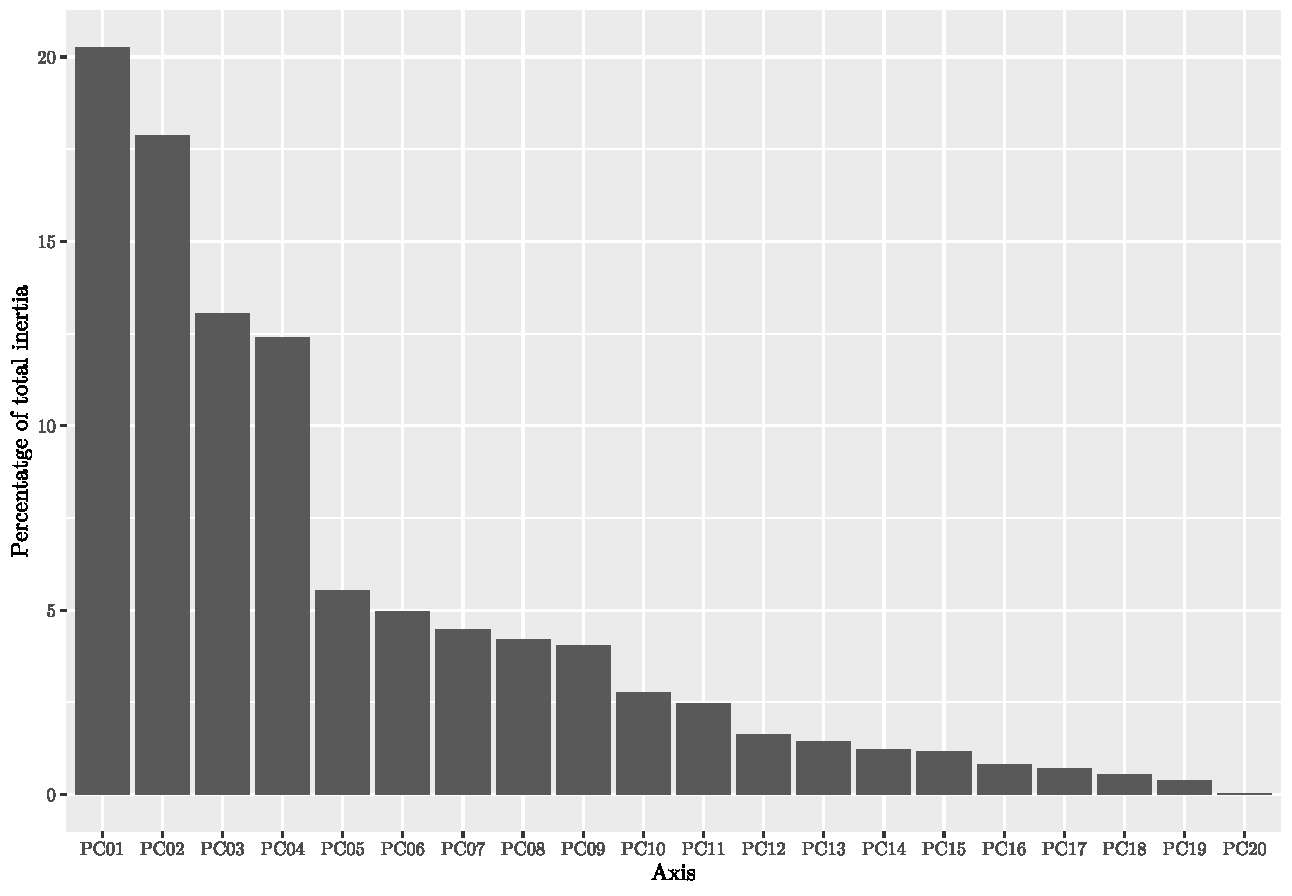
\includegraphics[width=0.7\linewidth]{PCA_inertia}
    \caption{PCA inertia}%
    \label{fig:pca_inertia}
\end{figure}

\begin{figure}[H]
    \centering
    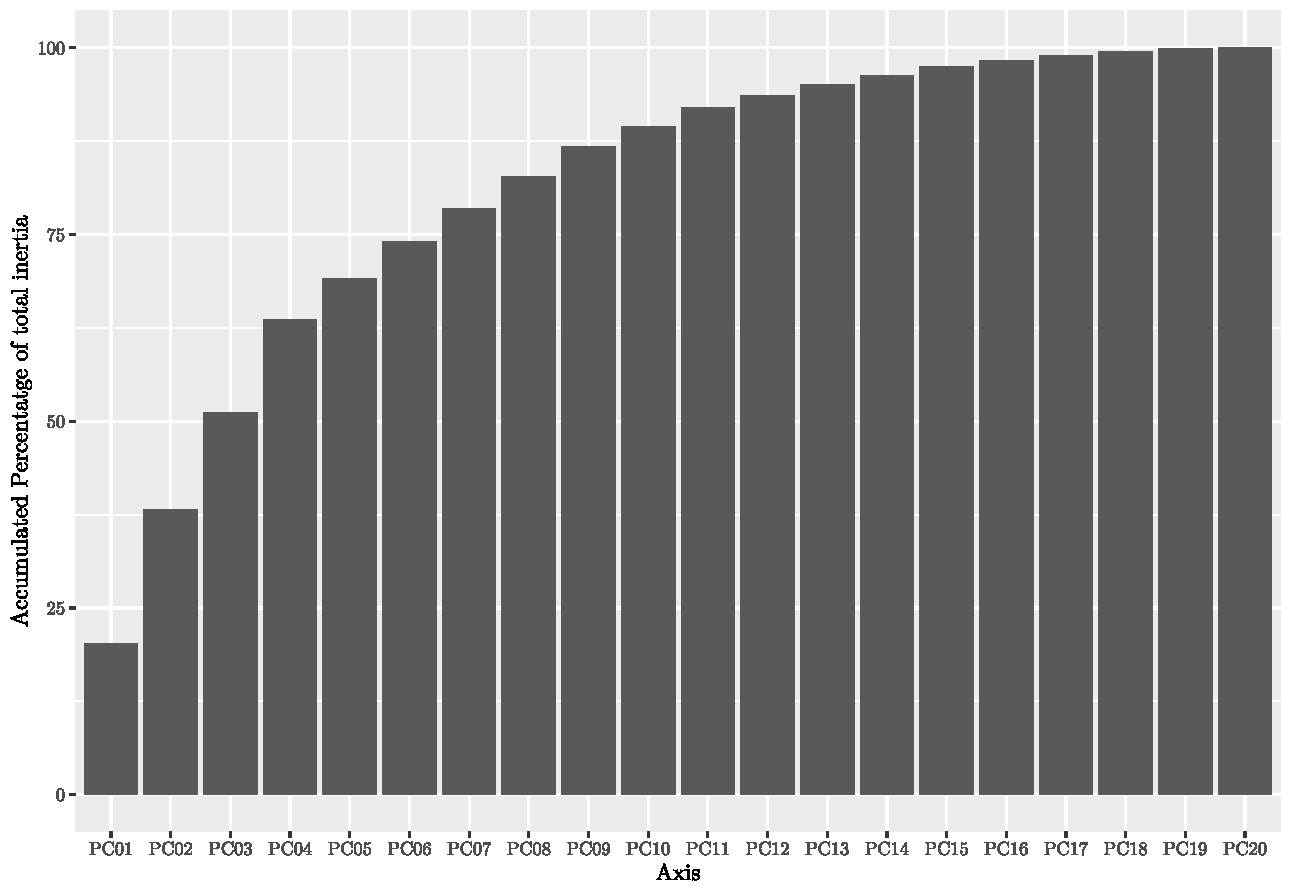
\includegraphics[width=0.7\linewidth]{PCA_inertia_cum}
    \caption{PCA accumulated inertia}%
    \label{fig:pca_inertia_cum}
\end{figure}

We used the inertia plots to decide the number of factorial axis to analyse. In plot \ref{fig:pca_inertia} we can conclude the 4 first axis represent a much larger amount of variance compared to the others. When looking at \ref{fig:pca_inertia_cum} we can see that the first 4 axis already contain 63\% of the variance. If we analyse further with the elbow method we can clearly see that the slop starts to decrease at around the 4th axis. Therefore we decided to only further analyse the first 4 factorial axis. 

% 20.24968405 17.88042469 13.04514781 12.39547495
% 20.24968  38.13011  51.17526  63.57073     %  69.09301  74.04671  78.51992  82.73880


% Factorial map visualisation:
\subsection{Factorial map visualisation}%
\label{sub:factorial_map_visualisation}

% #2 -> caption #3 -> file, #1 -> page
\newcommand{\factorialmap}[3][1]{
    \begin{figure}[H]
        \centering
        \includegraphics[width=0.85\linewidth,page=#1]{#3}
        \caption{#2}%
        \label{fig:#3-#1}
    \end{figure}
}

\begin{landscape}

%TODO
\factorialmap[3]{Test}{PCA_planes_sep}
\factorialmap[4]{Test}{PCA_planes_sep}

\end{landscape}

% (Be sure you use a single landscape pager for each single map in order to
% guarantee visibility of materials to the readers)

% For each factorial map provide:

% - Individuals projections

% - Common projection of numerical variables and modalities of qualitative
% - variables (take care to use correct color codes as explained along the course)

% - Interpretation of relationships among variables observed. When possible,
% - interpret the latent variable associated with the principal axis

% - Conclusions

% Note: All factorial maps must be placed in a single landscape page that makes
% it visible
